% Chapter 1

\chapter{Summative Evaluation} % Main chapter title

\label{summativeevalchapter} % For referencing the chapter elsewhere, use \ref{Chapter1} 

\lhead{Chapter \ref{summativeevalchapter}. \emph{Summative Evaluation}} % This is for the header on each page - perhaps a shortened title

%----------------------------------------------------------------------------------------
\section{Recruitment of Participants}
With help of a research assistant who was a resident of Langa,  we managed to recruit a total of fourteen adult participants (beneficiary users). We recruited these participants from two townships in Cape Town: Langa, and Athlone. In Langa there were five adult participants while in Athlone there were nine adult participants. The average age of these adult participants was 44.21 years with a standard deviation (S.D) of 9.99 years. The youngest adult was 26 years of age while the oldest was 60 years of age. Thirteen participants were females.\newline
Each adult participant (beneficiary user) elected one of their children/grand children to become their intermediary user to form a pair of users. The two members of a pair were required to work together in using the ``Family Wellness App'' to self-monitor the wellness of one member of a pair (a beneficiary user). All beneficiary users were working with their children but one whom was was working with her grand child.  The average age of children participants (intermediary users) was 15.42 (S.D=2.06) years. The youngest intermediary user was 12 years of age while the oldest was 20 years of age. The number of females and males intermediary users were equal.\newline
I gave out detailed information of what the study was all about to both intermediary and beneficiary participants. I informed them about different modes of which I will collect data. All beneficiary participants signed informed consent forms agreeing to be part of the study. Since all intermediaries were under 21 years of age, they signed assent forms which were also signed by their respective parents/guardians who were part of the study.\newline
One day was allocated for training intermediary participants on how to use the ``Family Wellness App''. In addition, each intermediary was given a user manual. After the training, I gave out one Android phone (Samsung GT-S5300) to each pair of participants. These phones were installed with two natives apps. The first app was a pedometer and the second one was the main ``Family Wellness App''. The ``Family Wellness App'' loaded all its content from a web application hosted remotely. Each beneficiary participants was required to carry the phone with them all the time in order for the pedometer app to count their steps. The two apps (main app and pedometer) were made available to the participants for a total period of six weeks. Each pair of participants provided the service provider's number of the SIM card that was inserted on their given Android phone. I allocated 1.3 GB of data to each SIM card. In addition each beneficiary participant was given a total of ZAR 240 as a compensation for transport and their time for the duration of the study. The details of the experiments are outlined on the next section.
\section{Experiments}
This phase of the study evaluated the effectiveness of gamification/rewards in motivating both intermediaries and beneficiaries to engage with the ``Family Wellness App''. I was comparing two versions of the applications. The first version of the application was simply a logbook or journal that allows each pair of users to record and view wellness data of a beneficiary member of a pair. With the logbook app, users could, view physical activity graphs, and recording and viewing summaries of nutrition components of food consumed by a beneficiary within a pair. The second version of the application was an extension of logbook  with an addition of a rewards/gamified subsystem. The experiments took place from the mid-October 2015 to the end of November 2015.  The details of how experiments were designed and how data were collected are presented on the next sub-section.
\subsection{Experiment Design}
The study used ``within-group'' design for the experiments. In within-group design, the same group of participants were exposed to different experimental conditions. This helps to minimize the number of groups needed to test hypotheses as only one group is used for both control and intervention. Another advantage of within-group design is that it minimizes the effect of confounding factors. The only problem with this approach is the learning effect and in addition, it lengthens duration of a study. In order to minimize the impact of the learning effect on the outcome, I randomly assigned pairs of participants to two separate groups referred to as experimental sequences. The first experimental sequence started with the ``Logbook App''  and finished with the ``Gamified App''. The second experimental sequence started with the ``Gamified App'' and finished with the ``Logbook App''. I used the following abbreviations ``LG'' and ``GL'' to refer to the first and second experimental sequences respectively.

A total of seven pairs of participants were assigned to the LG group while the remaining seven pairs were assigned to the GL group. Both groups spent the first four weeks in their first experimental conditions of which the ``Logbook App'' for the LG group and the ``Gamified App'' for the GL group. After 27 days (four weeks) each group was switched to a different experimental condition. The LG group started using the Gamified App while the GL group started using the Logbook App. The second phase of the experiment lasted for a total of 14 days (two weeks). 

The explanation of why four weeks in phase 1 and two weeks in phase 2 is as follows. Initially the plan was to have time spent on each experimental condition, be three(3) weeks intervals, but phase one had extended beyond three weeks up to fourth week as participants were not available for midline assessments at the end of the third week. Therefore, The research team carried out the assessment at the end of the fourth week and then followed by swapping of participants from one experimental condition to the other. This shortened the period for phase two from three to two weeks. Also, It was not feasible to extend phase two since it was approaching December of whereby most people travel for holidays, therefore, gathering participants during that time may have been impractical.
\subsection{Data Collection Methods and Analysis}
Data collection was a triangulation of application's logs,questionnaires and interviews. 
\subsubsection{Family Wellness App Logs}
Application's logs consisted of information regarding the time when there were users' activities on the app, the pair that was accessing the app at that time, and the functionality that was being accessed by that pair. Logs were categorized to their respective experimental conditions.  
Usage was measured by counting the number of sessions and clicks. A new session was defined as a period of detection of user's activity in an absence of any activity from this user/pair in the past one hour or more.\newline 
I carried out usage comparison in two dimensions. The first comparison entailed comparing the daily total number of sessions between the two experimental conditions for 41 days of experiments.\newline
In the second comparison, it was pairwise comparison of users' sessions in between logbook and gamification conditions. In order to ensure this comparison of usage is not affected by different experimental durations, I opted to use a relative number of unit measurement. In this case I used the number of sessions per day since the number of days on which pairs of users spent on a particular experimental condition differ between LG and GL group. For instance the LG group spent nearly four weeks in logbook and two weeks in gamification while the GL group spent four weeks in gamification and two weeks in logbook. In this second usage comparison, there were four pairs that were excluded from this usage analysis. These are pairs that faced hurdles on utilizing the app and this affected their ability to fully experience and engage with what was being offered by the gamified system. These pairs are listed on Table \ref{table:usageproblems}.\newline
\begin{table}[h!]
  \begin{center}
    \caption{Pairs with usability/technical problems that hinder their participation}
    \label{table:usageproblems}
	\begin{tabular}{|l|l|l|p{6cm}|}
		\hline
		&Pair&Experimental Sequence&Problem\\
		\hline
		1&Pair A&GL group &App not loading\\
		\hline
		2&Pair B&GL group&Lack of data bundles. \\
		\hline
		3&Pair C & LG group.& Pedometer never transmitted data to the server.\\
		\hline
		4&Pair D & LG group.& Pedometer stopped transmitting data to the server.\\
	\hline
	\end{tabular}
  \end{center}
\end{table}
\newline 
For \textbf{Pair A}, the app failed to load every time their intermediary user tried to use it. What was observed from the house where this pair lived in is that there was a poor Internet signal, hence the app was always failing to load most of the time. The second pair (\textbf{Pair B}), data was allocated to the wrong phone number at the beginning of experiments but they never reported on time. These two pairs (Pair A and Pair B) had the lowest usage days which were 2 and 3 days respectively and they they had used the app only in gamification condition.\newline
For the last two pairs (\textbf{Pairs C} and \textbf{D}) on Table \ref{table:usageproblems}, their pedometers were not transmitting steps' data to the server. Steps data were important for advancement of badges, and improvement of both the fish tank and botanical garden in gamification condition. Pair C's pedometer never transmitted any readings to the server even in logbook condition.  Pair D's pedometer stopped transmitting steps data on the fourth week of running the experiments and this was before this particular user was switched to gamification condition. The two intermediary users from Pair C and Pair D were close friends. Although the pedometer never transmitted data in Pair C  since the beginning of experiments, an intermediary user from this pair continued to use the wellness app because of the informal comparison with an intermediary user from Pair D while they were both still in logbook condition. The usage in Pair C and Pair D were both eleven days. Their drop out started during gamification condition. Pair C used the app for only three days and Pair D used it for only one day. Since gamification depended on transmission of steps to the server, pedometer problems affected Pair C and Pair D motivations to participate in gamification phase despite their efforts during logbook condition. The learning effect coupled with problems with their pedometers mediated their decrease in usage with the app.  An intermediary user from another pair in "LG" group who happened to live close to the Pair D and Pair C, shared her concerns about the rewards from the gamified app. This was during the endline interviews. This particular intermediary user didn't appreciate her advancement in badges because she admitted that her peers (the two intermediary users from Pair C and Pair D) did more efforts than her but they were not getting anything so she didn't understand why she was ahead of them. She was referring to their usage during logbook condition as they were both using the ``logbook App'' at the same time.  This proves that usability problems played a role to the some extent in demotivating participation in gamification condition  of intermediary users from Pair C and Pair D.
\subsubsection{Questionnaires}\label{methodsquestionnaire}
The reaserch team administered questionnaires at baseline, mid-line (during switching of experimental conditions), and end-line. The list of questionnaires is provided below.
\begin{enumerate}
\item{\textbf{Baseline Questionnaires}}\newline
At baseline both intermediary and beneficiary participants filled their respective questionnaires. 
\begin{itemize}
\item{\textbf{Intermediaries}}: Intermediaries participants' baseline questionnaire had three sections. The first section captured demographic information such as age,gender, and number services/apps used on cellphones. The second section included an IMI (Intrinsic Motivation Inventory) questionnaire  to assess participants' intrinsic motivation in using cellphones. The third section included an IMI questionnaire to assess participants' intrinsic motivation in helping their parents with cellphone based tasks.
\item{\textbf{Beneficiaries}}: Beneficiary participants' baseline questionnaire had four sections. The first section captured demographic information such as age,gender, and number services/apps used on cellphones. The second section included an IMI questionnaire to assess participants' intrinsic motivation in using cellphones. The third section included an IMI questionnaire to assess participants' intrinsic motivation in self-monitoring of diet/nutrition. The fourth section included an IMI questionnaire to assess participants' intrinsic motivation in self-monitoring of physical activity.
\end{itemize}
\item{\textbf{Midline Questionnaires}}\newline
Also at midline both intermediary and beneficiary participants filled their respective questionnaires. 
\begin{itemize}
\item{\textbf{Intermediaries}}: Intermediaries participants' midline questionnaire had only one section which included an IMI questionnaire  to assess participants' intrinsic motivation in using the family wellness app.
\item{\textbf{Beneficiaries}}: Beneficiary participants' baseline questionnaire had four sections. The first section included an IMI questionnaire  to assess participants' intrinsic motivation in using the family wellness app. The third section included an IMI questionnaire to assess participants' intrinsic motivation in self-monitoring of diet/nutrition. The fourth section included an IMI questionnaire to assess participants' intrinsic motivation in self-monitoring of physical activity.
\end{itemize}
\item{\textbf{Endline Questionnaires}}\newline
At endline both intermediary and beneficiary participants filled their respective questionnaires. 
\begin{itemize}
\item{\textbf{Intermediaries}}: Intermediaries participants' endline questionnaire had only one section which included an IMI questionnaire  to assess participants' intrinsic motivation in using the family wellness app.
\item{\textbf{Beneficiaries}}: Beneficiary participants' endline questionnaire had three sections. The first section included an IMI questionnaire  to assess participants' intrinsic motivation in using the family wellness app. The third section included an IMI questionnaire to assess participants' intrinsic motivation in self-monitoring of diet/nutrition.The fourth section included an IMI questionnaire to assess participants' intrinsic motivation in self-monitoring of physical activity.
\end{itemize}
\end{enumerate}
I developed the IMI questionnaires with the guidance of materials found on a ``Self-Determination Theory''\footnote{http://www.selfdeterminationtheory.org/intrinsic-motivation-inventory/} website which is maintained by researchers working on the theory including Richard Ryan and Edward Deci\citep{deci1985intrinsic} whom were early pioneers in developing the theory. I pretested these questionnaires during the informative evaluation of prototype II in chapter \ref{prototytpe2chapter}.  The most most important sub-scales for our theoretical construct were perceived competence and perceived autonomy which are part of the three basic psychological needs. The relatedness sub-scale is not yet validated but it was included in all questionnaires. Other sub-scale that was included in all questionnaires is perceived enjoyment. Perceived enjoyment is the only direct measure of intrinsic motivation while perceived competence and perceived autonomy are predictors of intrinsic motivation. Self-Determination theory suggests that a behaviour can be started as externally motivated and if external motivators support the three basic psychological needs which are relatedness, competitiveness, and autonomy then a behaviour that was once externally motivated can be internalized and users will start doing it because it is a good thing to do.\newline 
In addition to the aforementioned sub-scales, perceived usefulness and perceived efforts also appear in specific questionnaires (i.e self-monitoring of diet and activity, use of cellphone). These specific questionnaires don't assess specific constructs of self-determination theory as they focus on the overall intrinsic motivation. The overall IMI scores were computed by averaging the scores from each sub-scales.\newline 
In each question from the IMI sub scales, respondents were supposed to rate there experience in a scale of 1 to 7 points which means that 1 implies the statement is "not true at all" and 7 means the statement is "very true". \newline
There were three main objectives of using the IMI questionnaire. The first objective was to assess the ability of the two prototypes in supporting the participants with the three basic psychological needs. The difference in experimental durations was expected not to have any effect on motivations to use either of the two systems since both logbook and gamification were both present in both phases of experiments. Therefore, effects on motivations due to different durations were expected to cancel each other during analysis.\newline
The second objective of having IMI questionnaires was to use the overall IMI scores in assessing motivations of beneficiaries in self-monitoring of diet and activity, and motivations to use cellphone of both intermediaries and beneficiaries. These IMI questionnaires included perceptions of beneficiaries on competence, autonomy, relatedness, enjoyment, effort, and usefulness. I also examined motivation of intermediaries to help at baseline through a perceived enjoyment sub-scale of IMI questionnaire.\newline 
In motivations to self-monitor diet and activity, I excluded pairs (A,B, C, and D) from Table \ref{table:usageproblems} with problems that led to discontinuation of usage. In total only ten out of fourteen beneficiaries had their results included for analysis. In the comparison for self-monitoring of diet and activity, the first IMI comparison  entailed comparing the IMI score of each participant at baseline, midline, and endline regardless of an experimental condition. In the second comparison I compared scores at baseline, logbook, and gamification condition. The IMI score was computed from the average of all scores from sub-scales of perceived competence, perceived autonomy, perceived relatedness, perceived enjoyment, perceived effort,  and perceived usefulness. I  used one way ANOVA with repeated measures to test if there was a difference  between scores at: (1) baseline, midline, and endline, and (2)baseline, logbook and gamification. I used Mauchy's test\footnote{Read more on how Mauchy's test is used from http://www.statisticshell.com/docs/repeatedmeasures.pdf} to checked if different measuring points had the same covariance in each ANOVA test I carried out and this helped in deciding of whether to ``Sphericity Assumed'',``Greenhouse-Geisser'', or ``Huynh-Feldt'' of SPSS output.
\subsubsection{Interviews}
I also conducted short unstructured interviews at midline and endline. I selected fewer intermediaries and beneficiaries for the interviews. Interviews responses were important in supplementing data collected through questionnaires and application's logs.
\section{Findings}
There were four primary outcomes in analysing the findings and these are: (1)usage trend of the app; (2) user experience/intrinsic motivation  of both intermediaries and intermediaries in using the app; (3) intrinsic motivation of beneficiaries in self-monitoring of diet/nutrition; and (4) intrinsic motivation of beneficiaries in self-monitoring of physical activity.
\subsection{Usage Outcome}
The average number of days on which pairs used both versions of the application was 10.5 (SD=7.39) days. The most active usage was from a pair that utilized the app for a total of 26 days. The less active usage was from a pair that had used the app for only two days out of 41 days.\newline
\begin{figure}[htbp]
  \centering
    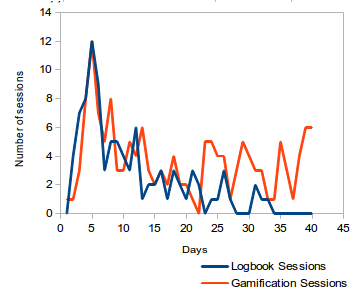
\includegraphics[width=0.6\textwidth]{Figures/scatter_daily_sessions.png}
    \rule{35em}{0.5pt}
  \caption{Total daily number of sessions from the two experimental conditions.}
  \label{figure:usagedailysessions}
\end{figure}\newline
Findings on comparison of daily total number sessions summed from all users in each experimental condition showed that gamification had a significant total number of daily sessions compared to logbook as demonstrated by a non-parametric test called Mann-Whitney U Test on Table \ref{table:usagedays}. I made a decision to use the aforementioned test because the two independent samples were not distributed normally (From ``\emph{Shapiro-Wilk Normality Test}''\footnote{http://sdittami.altervista.org/shapirotest/ShapiroTest.html}). Also, Figure \ref{figure:usagedailysessions} shows trends on total daily sessions in between logbook and gamification conditions. This finding shows that there is a higher likelihood of a gamified system to be used more frequent compared to a logbook system.\newline 
\begin{table}[h!]
  \begin{center}
    \caption{Daily usage comparison between Logbook and Gamified systems for 41 days}
    \label{table:usagedays}
	\begin{tabular}{|L{3cm}|c|c|c|c|c|c|}
		\hline
		Groups&N&Rank Average&Sum Ranks&U&Z&P\\
		\hline
   		Daily logbook sessions&41&33.72&1701.5&\multirow{2}{*}{1159.5}&\multirow{2}{*}{-2.9538}& \multirow{2}{*}{0.00318}\\\cline{1-4} 
   		 		    Daily gamification sessions&41&49.28& 1701.5&&&\\
\hline
	\end{tabular}
  \end{center}
\end{table}
The pairwise usage comparison on number sessions between users on  two experimental conditions which excluded four pairs showed that the Log mean of number of sessions per day was significantly higher on gamification condition, M=0.459; SD=0.336, when compared to logbook condition, M=0.201 ;SD=0.196 with (t(9)= -2.6593 ; p= 0.0261 ; 95\% CI=  -0.477 to -0.039). The finding above suggests that there was an indication of a significant increase in frequency of daily usage when pairs where in gamification condition. The log mean is used in this case because the differences of logbook and gamification didn't have a normal distribution shape. Therefore, I performed transformation using a natural logarithm equation and after transformations on the original data, the differences of the new data on logbook and gamification had a normal distribution shape.\newline
The utilization of different self-monitoring functionality on Figure \ref{figure:self_monitoring_usage}. showed that usage of some of the main self-monitoring features for steps and diet is lower in gamification compared to when in logbook condition. An explanation to this is that during  gamification condition users divided there attention between main logbook and virtual rewards. However, the trend in recording of diet/meals continued to remain the same between the two experimental conditions as the process of recording meals played an important role in earning some of the virtual rewards, therefore, intermediary users had to continue using that feature while in gamification condition. Figure \ref{figure:clicks_distr} shows the distribution of clicks among feedback features of the "Gamified Wellness App" and "The Logbook App".\newline 
\begin{figure}[htbp]
  \centering
    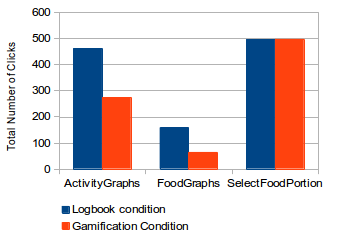
\includegraphics[width=0.6\textwidth]{Figures/self_monitoring_usage.png}
    \rule{35em}{0.5pt}
  \caption{Total clicks on feedback features for self-monitoring of wellness: ``Logbook App'' versus ``Gamified App''.}
  \label{figure:self_monitoring_usage}
\end{figure}\newline
\begin{figure}[htbp]
  \centering
    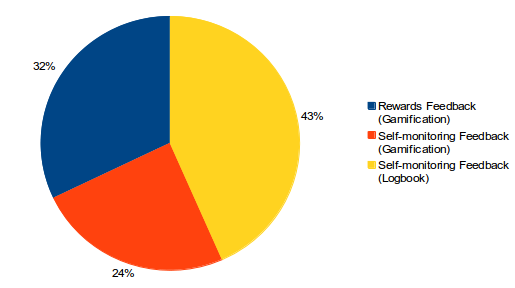
\includegraphics[width=0.45\textwidth]{Figures/clicks_distr.png}
    \rule{35em}{0.5pt}
  \caption{Total clicks on feedback features in the two experimental conditions : self-monitoring features versus rewards features.}
  \label{figure:clicks_distr}
\end{figure}\newline
From Figure \ref{figure:clicks_distr}, we can see that gamification condition's clicks on feedback features are distributed between the main self-monitoring and virtual rewards features. The number of clicks on the main self-monitoring feedback features had decreased as users became interested to feedbacks provided by virtual rewards features more than the main self-monitoring features.\newline
From Figure \ref{figure:usagedailysessions} above the trend shows the drop on Logbook condition as users who had been exposed to gamification condition before logbook condition became less interested with the "Logbook App" after being switched to it. The baseline data  can explain this usage information using descriptive trends since they were not statistically sufficient to explain the above usage. The drop in the total number of logbook sessions appears slightly the same in both younger and older intermediaries as shown on Figure \ref{figure:logbookbyage}.  But contrary to this is that younger intermediaries had slightly higher average on total number of sessions compared to the older ones while in gamification condition  as shown on Figure \ref{figure:gambyage}. Also on the average of total number sessions in both experimental conditions, the trend on average shows that younger intermediaries to have more sessions in overall as shown on Figure as more sessions were from gamification condition.  The term olerd and younger are defined by the age \textgreater= and \textless median age (15.5 years old) respectively.  Although the total number of sessions is relative to the number of days in which a pair of users had a particular experimental condition available to them, but younger and older intermediaries were evenly distributed to both experimental sequences (LG and GL groups). This means young and old intermediaries were both present in almost the same number in both experimental sequences hence their differences in number sessions which  is influenced by the number of days (27 days in phase 1 and 14 days in phase 2) are expected to cancel each other. The distribution by age group is presented on Table \ref{table:agregroupsall}.\newline 
\begin{figure}[htbp]
  \centering
    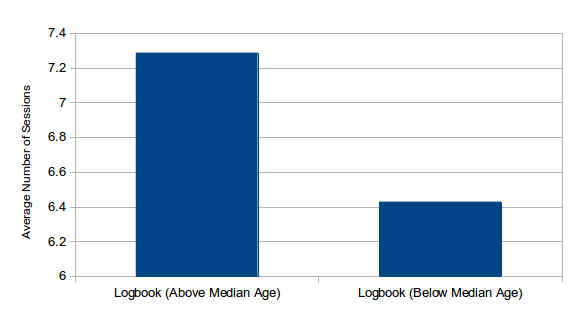
\includegraphics[width=0.5\textwidth]{Figures/logbookbyage.png}
    \rule{35em}{0.5pt}
  \caption{Average number of logbook sessions on  14 intermediaries: Age \textgreater= median age(=15.5) versus Age \textless median age.}
  \label{figure:logbookbyage}
\end{figure}\newline
\begin{figure}[htbp]
  \centering
    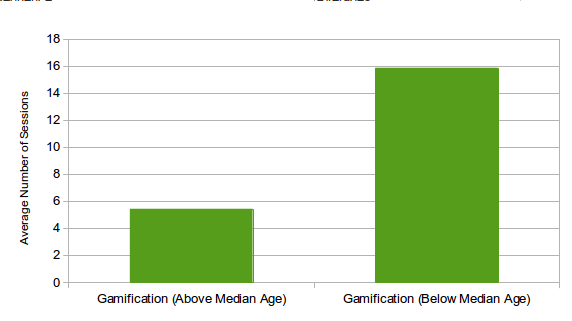
\includegraphics[width=0.5\textwidth]{Figures/gambyage.png}
    \rule{35em}{0.5pt}
  \caption{Average number of gamification sessions on  14 intermediaries: Age \textgreater= median age(=15.5) versus Age \textless median age.}
  \label{figure:gambyage}
\end{figure}\newline
\begin{figure}[htbp]
  \centering
    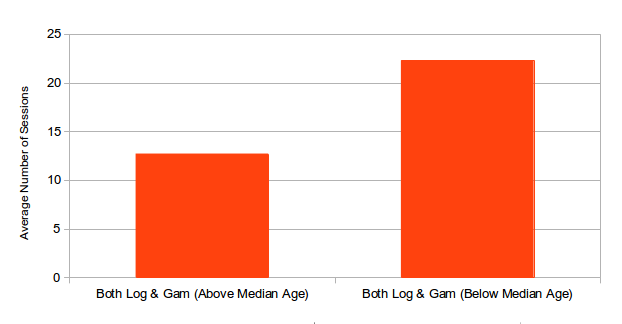
\includegraphics[width=0.5\textwidth]{Figures/bothexpebyage.png}
    \rule{35em}{0.5pt}
  \caption{Average of total number of sessions of  14 intermediaries on both experimental conditions: Age \textgreater= median age(=15.5) versus Age \textless median.}
  \label{figure:bothexpebyage}
\end{figure}
\begin{table}[h!]
  \begin{center}
    \caption{Age groups of intermediary participants}
    \label{table:agregroupsall}
	\begin{tabular}{|c|L{3.2cm}|L{1cm}|L{2cm}|L{2cm}|L{1.6cm}|L{1.3cm}|}
    		\hline
         &\textbf{Age Groups}&\textbf{Total users}&\textbf{No. of GL sequence}&\textbf{No. of LG sequence}&\textbf{No. of Females}&\textbf{No. of Males}\\
         \hline
         1&Age \textgreater=15.5 years&7&3&4&4&3\\  
\hline
         2&Age \textless15.5 years&7&4&3&3&4\\  
\hline
	\end{tabular}
  \end{center}
\end{table}\newline
For pairs who had usage problems on Table \ref{table:usageproblems},three out of four intermediary users were above the median age and one below age. A different trend that excludes the intermediary users that belong in these four pairs still appears to be similar to Figures \ref{figure:logbookbyage} and \ref{figure:gambyage}. For logbook condition, only intermediary users from Pairs A, B were removed as their participation as they terminated their early before switched to logbook condition. Pairs C and D started with Logbook and they participated through logbook conditions despite problems in Pair C since the beginning of experiments. Therefore, the new logbook trend only excluded pairs A, and B (Figures \ref{figure:logbookbyage_mod}). For the gamification condition, we removed pairs A,B,C, and D, as usage problems affected their ability to continue engaging with the app, therefore the new trend on average sessions is shown on Figure \ref{figure:gambyage_mod}\newline.
\begin{figure}[htbp]
  \centering
    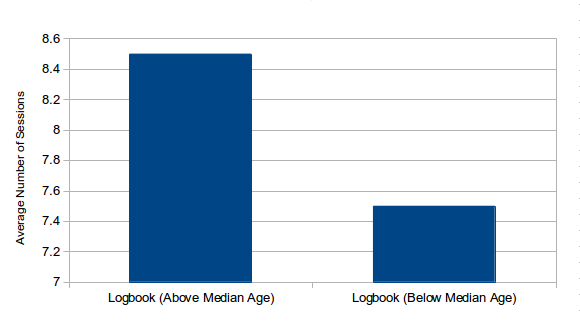
\includegraphics[width=0.5\textwidth]{Figures/logbookbyage_mod.png}
    \rule{35em}{0.5pt}
  \caption{Average number of logbook sessions on  12 intermediaries: Age \textgreater= median age(=15.5) versus Age \textless median age.}
  \label{figure:logbookbyage_mod}
\end{figure}\newline
\begin{figure}[htbp]
  \centering
    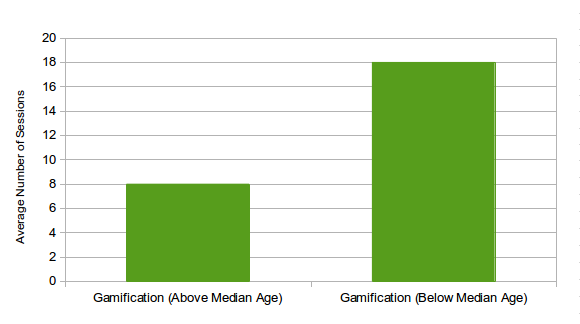
\includegraphics[width=0.5\textwidth]{Figures/gambyage_mod.png}
    \rule{35em}{0.5pt}
  \caption{Average number of gamification sessions on  10 intermediaries: Age \textgreater= median age(=15.5) versus Age \textless median age.}
  \label{figure:gambyage_mod}
\end{figure}\newline
The same trends continue to hold as younger intermediaries appear to have higher average number sessions in gamification condition and lower average number of sessions in logbook condition. Koivisto and Hamari \cite{koivisto2014demographic} found that the usage of  a gamified system is highly affected by the novelty effect which is inversely proportional to the age of participants, meaning that highly usage due to the novelty effect may be reported in much younger participants.\newline
The next trend is just looking at usage with respect to both ages of beneficiaries and intermediaries.  If we consider all beneficiary users from all fourteen pairs then the trend on average number of sessions is as shown on Figure \ref{figure:pairs_usage_sessions}. The median age for intermediaries was 15.5 years old while the median age for beneficiaries was 44 years old. Therefore an individual participant belongs to either younger or older group depending on whether ones age is below or above their respective median age. Pairs with a combination of a younger intermediary, and younger beneficiary appears to have more sessions in average. Most of these sessions were contributed by gamification.\newline 
\begin{figure}[htbp]
  \centering
    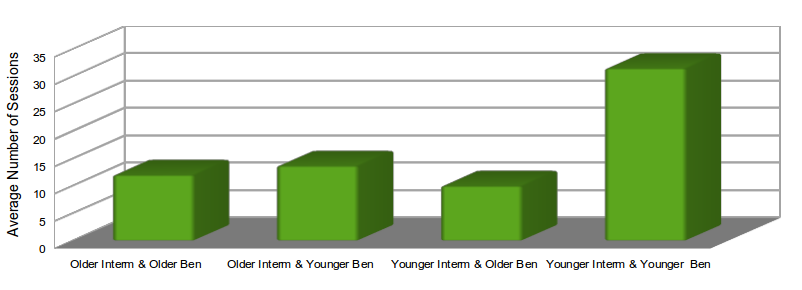
\includegraphics[width=0.6\textwidth]{Figures/pairs_usage_sessions.png}
    \rule{35em}{0.5pt}
  \caption{Average number of sessions on  14 pairs by age groups: intermediaries and beneficiaries}
  \label{figure:pairs_usage_sessions}
\end{figure}\newline
On the next sub sections, user experiences of both intermediaries and beneficiaries are reported.
\subsection{User Experience of Intermediaries}
Most of the time, beneficiaries' usage of the app was facilitated by intermediaries in proximate enabling and proximate translation. These types of intermediated interactions have been discussed in the work by Sambasivan et al.\cite{sambasivan2010}. Baseline data indicated that interest of intermediary participants in using cellphones was higher than that beneficiary participants. For instance, in overall IMI scores to use cellphone, intermediaries (M=5.76, S.D= 0.41, N=14) scored  significantly higher than beneficiary participants (M=5.06, S.D= 0.71, N=13) with (t(25)= 3.1764, p=0.0039, 95\% CI = 0.2472 to 1.1589).\newline
In user experience of intermediaries, the first finding is on how baseline intrinsic motivation and  demographic information such as age of intermediary users influenced user experience. From Figure \ref{figure:bothexpebyage} above, young intermediaries (age\textless median=15.5 years) appeared to had more number of sessions per day on average, but contrary to this trend was that, at baseline the average perceived enjoyment on helping with cellphone related tasks was higher in intermediaries with age\textgreater=median compared to intermediaries with age\textless median for the 12 intermediary users as shown on Figure \ref{figure:PE_HELP_Age}. 
\begin{figure}[htbp]
  \centering
    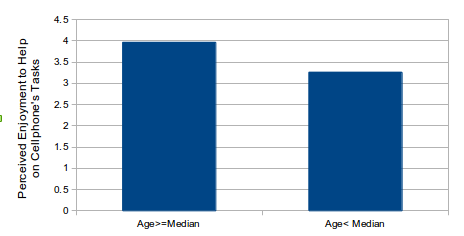
\includegraphics[width=0.5\textwidth]{Figures/PE_HELP_Age.png}
    \rule{35em}{0.5pt}
  \caption{Intermediaries' average perceived enjoyment to help others with cellphone tasks versus age group.}
  \label{figure:PE_HELP_Age}
\end{figure}\newline
The descriptive finding on perceived enjoyment to use the family wellness app by age at midline and endline for the 12 intermediary users (excluding users from pairs A and B since they terminated their usage too soon) showed that the averages are higher on the intermediaries with age \textless median for both midline and endline points (Figure \ref{figure:PE_Interm_App}). If we split the two age groups by, participants with different characteristics are evenly present to both groups as shown on Table \ref{table:agegroups}. Therefore, comparison of trends by age groups in not much influenced by other factors such the experimental sequence of which participants were assigned to or gender.\newline 
\begin{figure}[htbp]
  \centering
    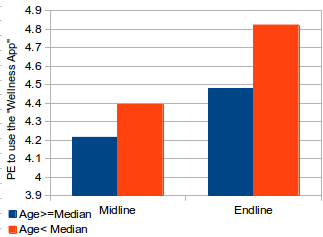
\includegraphics[width=0.5\textwidth]{Figures/PE_Interm_App.png}
    \rule{35em}{0.5pt}
  \caption{Intermediaries' average perceived enjoyment in using the app versus age group.}
  \label{figure:PE_Interm_App}
\end{figure}\newline
\begin{table}[h!]
  \begin{center}
    \caption{Age groups of intermediary participants}
    \label{table:agegroups}
	\begin{tabular}{|c|L{3.2cm}|L{1cm}|L{2cm}|L{2cm}|L{1.6cm}|L{1.3cm}|}
    		\hline
         &\textbf{Age Groups}&\textbf{Total users}&\textbf{No. of GL sequence}&\textbf{No. of LG sequence}&\textbf{No. of Females}&\textbf{No. of Males}\\
         \hline
         1&Age \textless 15.5 years&6&3&3&2&4\\  
\hline
         2&Age \textgreater=15.5 years&6&2&4&4&2\\  
\hline
	\end{tabular}
  \end{center}
\end{table}\newline
The trend on average perceived enjoyment in both logbook and gamified conditions appeared to be slightly higher in younger intermediaries compared to older intermediaries as shown on Figure \ref{figure:PE_Interm_App_exp_seq}. 
\begin{figure}[htbp]
  \centering
    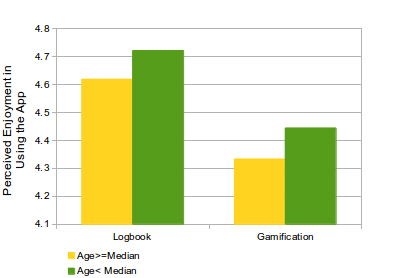
\includegraphics[width=0.5\textwidth]{Figures/PE_Interm_App_exp_seq.png}
    \rule{35em}{0.5pt}
  \caption{Intermediaries' average perceived enjoyment in using the app versus age group (Logbook and Gamification).}
  \label{figure:PE_Interm_App_exp_seq}
\end{figure}\newline
Figures \ref{figure:PE_Interm_App} and \ref{figure:PE_Interm_App_exp_seq}  suggest that the task of helping was more interesting to younger intermediaries due to the existence of the aforementioned motivational affordances.
There several factors that influence intermediaries to use the app and these are:
\begin{enumerate}
\item{\textbf{Self-monitoring task and the phone effect}}: The task itself of self-monitoring without rewards sparked interests of some intermediary users. This might be as the result of the novelty effect of visualization mechanisms and playfulness of users within a pair when they converse about what is happening on information presented by self-monitoring. This phenomenon of playfulness was observed in the previous chapter during evaluation of the second prototype (Chapter \ref{prototytpe2chapter}). Also the phone has an impact as intermediaries also skipped from the app to engage with other apps such as social media sites and games. Users switched to different apps.
\item{\textbf{Informal comparisons}}: Comparison on steps graphs can be another source motivation. For intermediaries who were close, they did this form of informal comparison. In the absence of gamification, still intermediaries thought that they were competing with other therefore those who were close had face to face interactions of where they did comparison with one another.
\item{\textbf{Gamification comparison}}: This kind of comparison increased the number of times intermediary user checked the app.
 The ``Gamified App'' was designed in such a way that a pair will earn rewards based on usage and the average number of steps walked by a beneficiary participant who is a member of the pair. The purpose of rewards was to foster users' intrinsic experiences such as competitiveness and a sense of autonomy which are predictors of intrinsic motivation. Rewards depended on four parameters and these were the number of steps walked by a beneficiary user, the number of days the app has been used by an intermediary to either to record meals or to view feedback on meals, points, steps, gardens, etc. During interviews, I discovered that in one pair not only the beneficiary was using the pedometer, an intermediary was also taking turns to use the pedometer, therefore they were collaborating in accumulating steps. Both an intermediary user and a beneficiary user had discussions of whether the person whose turn it was had walk enough steps. They did this to accumulate more steps than other pairs. In addition to comparison other intermediary users came to the app to the gamified app to connect to other users.
\item{\textbf{Requests from beneficiary users}}:There were times where intermediary users engaged with the app only upon receiving requests from beneficiaries. Intermediaries were interested to fulfil requests from beneficiaries provided an intermediary was interested with the self-monitoring task; steps comparison; or gamification comparison. 
\end{enumerate} 
Interest of intermediaries varied as some valued more on the social relatedness brought by the intervention while other where concerned about achievement (i.e. dominating others in competitions). Gamification appeared to be the most dominant factor that influenced usage as we have already seen that the frequency of usage showed a higher value in gamification when compared to logbook.\newline
However, not all intermediaries had a positive user experience on utilizing gamification, that is why the average perceived enjoyment appears to be lower for both age groups while in gamification condition compared to the logbook condition (Figure \ref{figure:PE_Interm_App_exp_seq}). If we go back we can see that four pairs had usage problems as mentioned on Table \ref{table:usageproblems}.  From those four pairs, two pairs had severe usability problems and these were pair A and Pair C. Pair B tried to use the app a few times but since they didn't have data bundles usage was terminated immediately, however, the continued to receive SMS feedback throughout the experimental conditions of which some of it was positive as they had managed to attain some badges. User from pair D also appeared to be more interested during gamification even though he terminated usage after his first week on gamification.  We can see that problems in this pair only started on the fourth week of logbook condition (one week before switching to gamification condition), therefore, the  with the pedometer didn't affect much the motivation of the intermediary user from Pair D as he enjoyed the gamification condition despite the fact that he logged in once throughout this experimental condition and the pedometer was not transmitting data to the server. The two users from Pair B and Pair D, had their motivation not affected by usability problems as for Pairs A and C. SMS feedbacks and reminders were sent to all fourteen pairs and this some how engaged users from Pair B and Pair D. During gamification, if a particular pair managed to acquire a new badge, all other pairs were notified through SMS including the pair that had attained a badge. In addition intermediaries were reminded of what has been done and what remains to be done in order to attain higher badges. During logbook condition, intermediaries were notified with SMS of how many steps have been walked by their intermediary so far and they were also reminded that to assist their beneficiaries in monitoring their wellness. Therefore since, usability problems in Pair B and D were not severe as for pairs A and C, and combination of text messages feedbacks, motivation of users in pairs D, and C appeared to be slightly higher in gamification condition compared to logbook condition. From here we can conclude that Pairs A and C motivations during gamification condition were negatively affected by the severe usability problems.\newline 
Gamification condition didn't harm motivation of only users with severe usability problems. There was  a very intriguing phenomenon from two other intermediary users from \textbf{Pair E} and \textbf{Pair F} as mentioned on Table \ref{table:negexprnce}. The two intermediary users had used the app more often in gamification condition  compared to when they were in logbook condition but had reported both lower scores in perceived enjoyment, and perceived competence when in gamified condition compared to when they were in logbook condition. Two of these intermediary users were  in LG and GL groups respectively. I examined the performance of these two users in gamification rewards and discovered that two users never managed to make any progress in attaining a single reward despite their efforts in using the ``Gamified App''. This harmed both their perceived enjoyment and perceived competence to use the "Family Wellness App" while in gamification condition. One of these two intermediary participants sent an SMS to the researcher asking what he was supposed to do in order to advance in badges and he was informed that all the information was specified in their given user manual. In addition, SMS reminders were sent out to all intermediaries to inform them of how far they have gone in achieving rewards and what is remaining in terms of usage and steps in order for them to reach the next badge. Their beneficiary participants were not walking enough steps despite the fact that these intermediaries had put  more efforts in using the App during gamification condition. Badges were earned in combination of both the app usage and average number of steps walked by a beneficiary user. One beneficiary who was working with one of these intermediary users also reported in interviews that there was always a contention with her intermediary when this beneficiary wanted to see what was going in the app as the intermediary was not voluntarily willing to help some of the time.\newline
\begin{table}
  \begin{center}
    \caption{Pairs affected by poor design of gamification}
    \label{table:negexprnce}
	\begin{tabular}{|L{1cm}|L{1.5cm}|L{2.2cm}|L{8cm}|}
		\hline
		&Pair& Experimental Sequence&Challenge\\
		\hline
		1&Pair E&LG group & The beneficiary participant was not walking enough steps hence impacted performance in gamification\\
		\hline
		2&Pair F & LG group.& Same as above.\\
	\hline
	\end{tabular}
  \end{center}
\end{table}
\newline   
Therefore the conclusion was that, the two intermediary users on Table \ref{table:negexprnce}  had a negative experience as the result of failure of our gamification design to match challenges with abilities. i.e. efforts of beneficiaries differed hence challenges should have matched with individual abilities of beneficiaries within pairs. When challenges are too difficult as they don't match users' skills, end users can become demotivated \citep{zhang2008motivational}. As result only eight intermediary users were considered in the main sub scales of intrinsic motivation (autonomy, competence, and enjoyment).\newline
I compared between the ability of the two prototypes in affording three basic psychological needs suggested by self-determination theory. In addition, I also included perceptions on enjoyment as it is a direct measure of intrinsic motivation. The corresponding scales from the IMI questionnaire were administered at midline and endline . Therefore, there were four sub-scales; perceived competence, perceived autonomy, perceived enjoyment and perceived relatedness.  For the reason I stated above, I decided to exclude users from  Pair A and C on Table \ref{table:usageproblems} , and Pairs E and F on Table \ref{table:negexprnce}. A total of ten pairs were considered for analysis on the aforementioned intrinsic motivation sub-scales.\newline
The hypotheses of interest for intermediaries were:
\begin{enumerate}
\item{Hypothesis 1}
\begin{itemize}
\item{H\SB{0}}:There is no difference in perceived competence in using the app between a logbook app and gamified app
\item{H\SB{A}}:There is a difference in perceived competence in using the app between a logbook app and gamified app
\end{itemize}
\item{Hypothesis 1}
\begin{itemize}
\item{H\SB{0}}:There is no difference in perceived autonomy in using the app between a logbook app and gamified app
\item{H\SB{A}}:There is a difference in perceived autonomy in using the app between a logbook app and gamified app
\end{itemize}
\item{Hypothesis 3}
\begin{itemize}
\item{H\SB{0}}:There is no difference in perceived enjoyment in using the app between a logbook app and gamified app
\item{H\SB{A}}:There is a difference in perceived enjoyment in using the app between a logbook app and gamified app
\end{itemize}
\item{Hypothesis 4}
\begin{itemize}
\item{H\SB{0}}:There is no difference in perceived relatedness in using the app between a logbook app and gamified app
\item{H\SB{A}}:There is a difference in perceived relatedness in using the app between a logbook app and gamified app
\end{itemize}
\end{enumerate}
The findings (Table \ref{table:imiwellnessinterm}) indicate that perceived competence of intermediaries in using the ``Family Wellness App'' was significantly higher in the gamified condition than in the logbook condition in the ten intermediaries that were analysed. Perceived autonomy, perceived enjoyment, and perceived relatedness were all not different between gamification condition and logbook condition. For perceived enjoyment and autonomy, there are cases were the self-monitoring task was interesting enough on itself or when combined with informal comparison of steps among intermediary users. Therefore, there some intermediaries who felt more enjoyment while they were in logbook condition, which is also the same case for perceived autonomy. For perceived relatedness, the app brought users together regardless of an experimental condition especially the ones that already knew each other before. Therefore increase in relatedness happened in both versions of the prototype.\newline
\begin{table}[h!]
  \begin{center}
    \caption{Comparison of ten intermediaries' scores on sub-scales of competence, autonomy, enjoyment, and relatedness in using the ``Family Wellness App}
    \label{table:imiwellnessinterm}
	\begin{tabular}{|c|c|c|}
		\hline
		Mean &Logbook App&Gamified App\\
		\hline
		 \multirow{2}{*}{Perceived competence}&M=5.23; SD=1.02&M=5.96; SD=0.66\\\cline{2-3} 

		 &\multicolumn{2}{|l|}{t(9)=-3.4949; p=0.0068 ; 95\% CI= -1.204 to -0.258} \\
\hline
		 \multirow{2}{*}{Perceived autonomy}&M=3.95; SD=0.86&M=3.96; SD=0.94\\\cline{2-3} 

		 &\multicolumn{2}{|l|}{t(9)= -0.0269; p= 0.9792; 95\% CI= -0.596 to 0.582} \\
\hline
		 \multirow{2}{*}{Perceived enjoyment}&M=4.18; SD=1.11&M=4.75; SD=1.32\\\cline{2-3} 

		 &\multicolumn{2}{|l|}{t(9)=-1.6930;  p=0.1247; ; 95\% CI= -1.343 to 0.193 } \\
\hline
		 \multirow{2}{*}{Perceived relatedness}&M=4.22; SD=0.63&M=4.37; SD=0.9\\\cline{2-3} 
		 &\multicolumn{2}{|l|}{t(9)= -0.7193; p=0.4902; 95\% CI= -0.622 to 0.322 } \\
\hline
	\end{tabular}
  \end{center}
\end{table}
\subsection{User Experience of Beneficiaries}
As most beneficiaries only interfaced with the app through intermediary users, beneficiaries' user experience relied on cooperation they got from intermediaries. There cases were beneficiaries had a negative experience as result of intermediaries refusing to assist upon being given requests. This happened in cases of where intermediary users didn't feel like helping because of other tasks. An overall motivation show that most beneficiaries were excited about engaging with their personal information. In addition to that, from Figure \ref{figure:pairs_usage_sessions}, a combination of younger intermediary and beneficiary users had more sessions in average and this is because gamification influenced younger intermediary users to use the app, while it also influenced younger beneficiaries to pass their requests to their respective intermediaries more often. For instance in interviewing one pair that consisted of a younger intermediary and beneficiary users, this pair had highest number of sessions in gamification. In the course of using the app they both exhibited playfulness behaviours in engaging with gamification of whereby they discussed strategies about beating other teams. So every time a beneficiary user from this pair would request her intermediary to open the app so that she can see if they are ahead of other teams.\newline
Older intermediaries were not so much into gamification. What pushed them to use the app was more of both requests from their beneficiaries and their sense being more accountable to help. Therefore older intermediaries may have more empathy of why they are helping compared to younger intermediaries. So in this scenario, older intermediaries' usage may depend mostly on motivation of beneficiaries to request help while for young intermediaries, gamification may be a driving factor but beneficiaries need to be motivated too in order for intermediaries to be enthusiastic to share information with them.\newline
In the next sub-section, the IMIs in self-monitoring of diet and activity are reported. Four pairs with usage problems (Table \ref{table:usageproblems}) were excluded.\newline
\subsubsection{IMI in Self-Monitoring of Diet}
The results on self-monitoring of diet (baseline, midline, and endline) are shown on Table  \ref{table:imidietbenf}. The Mauchly’s test indicated that the assumption of sphericity was not violated with  $\chi{}$\SP{2}(2)=3.76, p=0.152. The results (N=10) on  ``Self-monitoring of Diet'' shown on Table \ref{table:imidietbenf} were from ``Sphericity Assumed'' output. ANOVA showed that there was a significant difference of average IMI scores on self-monitoring of diet measured at baseline, midline and endline.
\begin{table}[h!]
  \begin{center}
    \caption{Comparison of ten beneficiaries' IMI scores in self-monitoring of diet at baseline, midline and endline}
    \label{table:imidietbenf}
	\begin{tabular}{|L{2.8cm}|L{3.2cm}|L{3.2cm}|L{3.2cm}|}
		\hline
		Mean IMI Score &Baseline&Midline&Endline\\
		\hline
		 %\multirow{3}{*}
		 {Self-monitoring}&M=4.48; SD=1.24&M=5.07; SD=1.19;&M=5.55; SD=0.95\\\cline{2-4} 

		of Diet &\multicolumn{3}{|l|}{F(2,18)=3.787; p=0.042} \\
\hline	\end{tabular}
  \end{center}
\end{table}
A finding from a pairwise comparisons (a paired student t-test) indicated that the IMI score at endline was significantly higher than at baseline (Table \ref{table:imipairwisediet}). There was no significant difference on baseline versus midline and midline versus endline (Tables \ref{table:imipairwisediet1}, and \ref{table:imipairwisediet2}). Motivation to self-monitor diet appeared to increase with time as shown on Figure \ref{figure:imi_diet}. The interpretation of the above findings are that the wellness app appeared to had a significant effect of time on motivation of beneficiaries to self-monitor their diet.\newline
\begin{table}[h!]
  \begin{center}
    \caption{Pairwise comparisons of IMI scores in self-monitoring of diet: Baseline versus Midline}
    \label{table:imipairwisediet}
	\begin{tabular}{|L{2cm}|L{4cm}|L{4cm}|}
		\hline
		Mean &Baseline&Midline\\
		\hline
		 \multirow{2}{*}{IMI Score}&M=4.48; SD=1.24&M=5.07; SD=1.19\\\cline{2-3} 

		 &\multicolumn{2}{|l|}{t(9)=-1.298; p=0.227 ; 95\% CI= -1.621 to 0.439} \\
\hline
	\end{tabular}
  \end{center}
\end{table}
\begin{table}[h!]
  \begin{center}
    \caption{Pairwise comparisons of IMI scores in self-monitoring of diet: Baseline versus Endline}
    \label{table:imipairwisediet1}
	\begin{tabular}{|L{2cm}|L{4cm}|L{4cm}|}
		\hline
		Mean &Baseline&Endline\\
		\hline
		 \multirow{2}{*}{IMI Score}&M=4.48; SD=1.24&M=5.55; SD=0.95\\\cline{2-3} 

		 &\multicolumn{2}{|l|}{t(9)=-2.457; p=0.036 ; 95\% CI= -2.06083 to -0.08517} \\
\hline
	\end{tabular}
  \end{center}
\end{table}
\begin{table}[h!]
  \begin{center}
    \caption{Pairwise comparisons of IMI scores in self-monitoring of diet: Midline versus Endline}
    \label{table:imipairwisediet2}
	\begin{tabular}{|L{2cm}|L{4cm}|L{4cm}|}
		\hline
		Mean &Midline&Endline\\
		\hline
		 \multirow{2}{*}{IMI Score}&M=5.07; SD=1.19&M=5.55; SD=0.95\\\cline{2-3} 

		 &\multicolumn{2}{|l|}{t(9)=-1.975; p=0.08 ; 95\% CI= -1.0342 to 0.07017} \\
\hline
	\end{tabular}
  \end{center}
\end{table}
\newline
\begin{figure}[htbp]
  \centering
    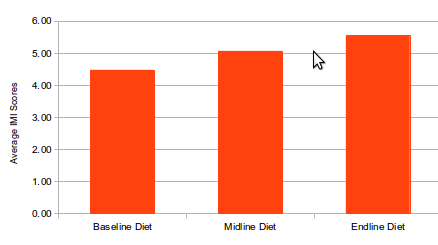
\includegraphics[width=0.4\textwidth]{Figures/imi_diet.png}
    \rule{35em}{0.5pt}
  \caption{Trend on Average IMI Scores of Self-Monitoring of Diet at Baseline, Midline, and Endline.}
  \label{figure:imi_diet}
\end{figure}\newline
The aforementioned ANOVA finding on comparison among baseline, midline, and endline doesn't discern between different experimental conditions of which pairs of users were exposed to. The ANOVA finding (N=10)(Table  \ref{table:imidietbenf2}) on the comparison of IMI scores to self-monitor diet, among baseline, logbook, and gamification conditions showed that there was no significant difference of average IMI scores on self-monitoring of diet measured during baseline, logbook and gamification conditions. This finding is from the ``Sphericity Assumed'' output of the ANOVA test since the Mauchly’s test indicated that the assumption of sphericity was not violated with  $\chi{}$\SP{2}(2)=2.19, p=0.335. The trend on averages shows both logbook and gamification to be slightly higher than baseline as shown on Figure \ref{figure:imi_diet2}. The conclusion from this finding is that both versions of the prototype have shown an indication of increasing motivation of beneficiaries to self-monitor diet.\newline
\begin{table}[h!]
  \begin{center}
    \caption{Comparison of ten beneficiaries' IMI scores in self-monitoring of diet at baseline, after logbook, and  after gamification conditions}
    \label{table:imidietbenf2}
	\begin{tabular}{|L{2.8cm}|L{2.5cm}|L{2.5cm}|L{2.5cm}|}
		\hline
		Mean IMI Score &Baseline&Logbook&Gamification\\
		\hline
		 %\multirow{3}{*}
		 Self-monitoring&M=4.48; SD=1.241&M=5.28; SD=1.05&M=5.34; SD=1.16\\\cline{2-4} 
		 of Diet&\multicolumn{3}{|l|}{F(2,18)=3.787; p=0.087} \\
\hline	\end{tabular}
  \end{center}
\end{table}\newline
\begin{figure}[htbp]
  \centering
    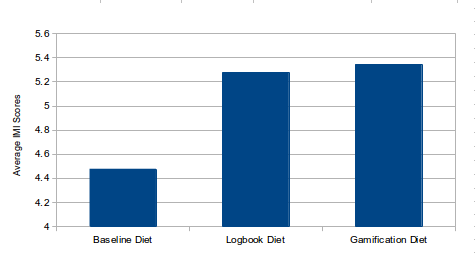
\includegraphics[width=0.4\textwidth]{Figures/imi_diet2.png}
    \rule{35em}{0.5pt}
  \caption{Trend on Average IMI Scores of Self-Monitoring of Diet at Baseline, Logbook, and Gamification.}
  \label{figure:imi_diet2}
\end{figure}\newline
\subsubsection{IMI in Self-Monitoring of Activity}
The results (N=9) on self-monitoring of activity are shown on Table  \ref{table:imiactivitybenf}. The results are based on a sample of nine beneficiary users as one participant didn't complete this part of the questionnaire at baseline.  The Mauchly’s test indicated that the assumption of sphericity was violated with  $\chi{}$\SP{2}(2)=8.248, p=0.016. The value $\epsilon$ on Greenhouse Geisser was ``\textless 0.75'', therefore, the results on  ``Self-monitoring of Diet'' shown on Table \ref{table:imiactivitybenf} were selected from ``Greenhouse-Geisser'' output. ANOVA showed that there was no significant difference of average IMI scores on self-monitoring of activity measured at baseline, midline and endline. The trend of means appears to increase from baseline to endline as shown on Figure \ref{figure:imi_activity}.\newline
There are several factors that could have contributed to results not being significant among baseline, midline,endline points,. The first hypothesized reason is tracking of physical activity appeared to be easy in majority of the participants even without tracking devices as people can estimate the distance they walk daily and they consider this as tracking even though they might have means to record this information, hence their motivation was high at baseline unlike diet self-monitoring which they consider it to be cumbersome due to external barriers such as health food being expensive, therefore at baseline participants felt more motivated to track their activity. The second hypothesized reason is that the sample size was small hence there was a smaller power in detecting significant difference. But we have seen that the trend in motivation increases with time.\newline 
\begin{table}[h!]
  \begin{center}
    \caption{Comparison of ten beneficiaries' IMI scores in self-monitoring of activity at baseline, midline and endline}
    \label{table:imiactivitybenf}
	\begin{tabular}{|L{2.8cm}|L{2.5cm}|L{2.5cm}|L{2.5cm}|}
		\hline
		Mean IMI Score &Baseline&Midline&Endline\\
		\hline
		 %\multirow{3}{*}
		 Self-monitoring&M=4.82; SD=1.002&M=5.28; SD=1.003&M=5.41; SD=0.894\\\cline{2-4} 
		 of activity&\multicolumn{3}{|l|}{F(1.182, 9.455)=2.936; p=0.116} \\
\hline	\end{tabular}
  \end{center}
\end{table}\newline
\begin{figure}[htbp]
  \centering
    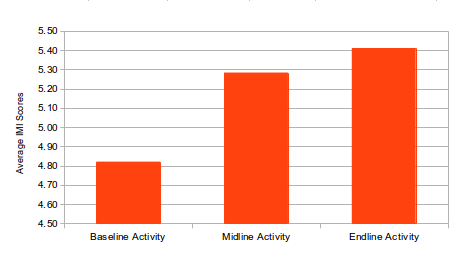
\includegraphics[width=0.4\textwidth]{Figures/imi_activity.png}
    \rule{35em}{0.5pt}
  \caption{Trend on Average IMI Scores of Self-Monitoring of Activity at Baseline, Logbook, and Gamification.}
  \label{figure:imi_activity}
\end{figure}\newline
The finding from an analysis (N=9) that examined if there is a difference among baseline,logbook, and gamification in self-monitoring of activity, showed that there was no significant difference of average IMI scores on self-monitoring of activity measured at baseline, logbook and gamification (Table {table:imiactivity2benf}). The Mauchly’s test indicated that the assumption of sphericity was violated with  $\chi{}$\SP{2}(2)=6.788, p =0.034. The value of $\epsilon$ on Greenhouse Geisser was ``\textless 0.75'', therefore, these results on  ``Self-monitoring of Activity'' were selected from ``Greenhouse-Geisser'' output of oen way with repeated measures ANOVA test. The trend in motivation increases in both logbook and gamification compared to baseline as shown on Figure \ref{figure:imi_activity2}\newline
%epsilon=0.617
\begin{table}[h!]
  \begin{center}
    \caption{Comparison of ten beneficiaries' IMI scores in self-monitoring of activity at baseline, logbook and gamification}
    \label{table:imiactivity2benf}
	\begin{tabular}{|L{2.8cm}|L{2.5cm}|L{2.5cm}|L{2.5cm}|}
		\hline
		Mean IMI Score &Baseline&Logbook&Gamification\\
		\hline
		 %\multirow{3}{*}
		 Self-monitoring&M=4.82; SD=1.002&M=5.33; SD=0.9762&M=5.37; SD=0.9276\\\cline{2-4} 
		 of activity&\multicolumn{3}{|l|}{F(1.234, 9.872)=2.783; p=0.123} \\
\hline	\end{tabular}
  \end{center}
\end{table}\newline
\begin{figure}[htbp]
  \centering
    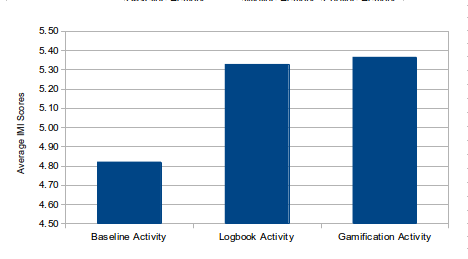
\includegraphics[width=0.4\textwidth]{Figures/imi_activity2.png}
    \rule{35em}{0.5pt}
  \caption{Trend on Average IMI Scores of Self-Monitoring of Activity at Baseline, Logbook, and Gamification.}
  \label{figure:imi_activity2}
\end{figure}\newline
\begin{flushright}
\end{flushright}

